%-------------------------------%
% Biblography
%------------------------------%
\RequirePackage{filecontents}        % loading package filecontents
% writing file \jobname.bib, for example mb-bibtex.bib.

\begin{filecontents*}{\jobname.bib}

@conference{,
%[A]
%[B]
@book{Bishop:06,
  title={Pattern recognition and machine learning},
  author={Christopher M Bishop},
  year={2006},
  publisher={Springer New York}
}

%[D]
@inproceedings{Das:08,
  title={Adapting to a Market Shock: Optimal Sequential Market-Making.},
  author={Das, Sanmay and Magdon-Ismail, Malik},
  booktitle={NIPS},
  pages={361--368},
  year={2008}
}
%[E]
%[F]
%[G]
%[H]
%[I]
%[J]
%[K]
@book{Keeney:93,
  title={Decisions with multiple objectives: preferences and value trade-offs},
  author={Keeney, Ralph L and Raiffa, Howard},
  year={1993},
  publisher={Cambridge university press.}% Original publication, Wiley, New York, 1976}
}

@book{Koller:09,
  title={Probabilistic graphical models: principles and techniques},
  author={Koller, Daphne and Friedman, Nir},
  year={2009},
  publisher={The MIT Press}
}
%[L]
%[N]
%[O]
%[P]
%[Q]
%[R]
%[S]
@conference{Sanner:12,
author = {Scott Sanner and Ehsan Abbasnejad},
title = {Symbolic Variable Elimination for Discrete and Continuous Graphical Models},
booktitle = {AAAI},
year = {2012}
}
%[T]
%[U]
%[V]
%[W]
%[X]
%[Y]
%[Z]

\end{filecontents*}

\documentclass{article} % For LaTeX2e
%\usepackage{nips13submit_e,times}%{nips13submit_e,times}
\usepackage{hyperref}
\usepackage{url}
\usepackage{amsthm} %for theorems, examples, etc.
\usepackage{amsfonts} %for matbb font
\usepackage{graphicx}
\usepackage{caption} %for graphics
\usepackage{subcaption} %for graphics
\usepackage{amsmath} %for cases

\usepackage{algorithmic} %for algorithms
% Import an algorithm formatting package
\usepackage[vlined,algoruled,titlenumbered,noend]{algorithm2e}
%\documentstyle[nips13submit_09,times,art10]{article} % For LaTeX 2.09
%\usepackage{algpseudocode} %new tpr
%\usepackage{algorithm} %new tpr

\usepackage{verbatim} %for commenting

%\newenvironment{proof}{{\noindent\bf Proof.}}\qed%{\hspace*{\fill}\ensuremath{\diamondsuit\quad}%{\vskip 1ex}
\newtheorem{theorem}{Theorem}
\newtheorem{proposition}{Proposition}
\newtheorem{example}{Example}
\def\fexample#1#2#3{\vspace{-1ex}\begin{example}[#2]\label{#1}\rm #3
\hspace*{\fill} $\diamondsuit\quad$ \end{example}\vspace{-2ex} }
\newcommand{\tuple}[1] {\langle #1 \rangle}
\newcommand{\bvec}[1]{\textbf{#1}}
\newcommand{\indicator}{\mathbb{I}}%{I\!\!I}

\def\eqvsp{}  \newdimen\paravsp  \paravsp=1.3ex
\def\paradot#1{\vspace{\paravsp plus 0.5\paravsp minus 0.5\paravsp}\noindent{\bf\boldmath{#1.}}}

\title{
%Blocked Gibbs Sampling on Piecewise Bayesian Networks
REPORT
}




% The \author macro works with any number of authors. There are two commands
% used to separate the names and addresses of multiple authors: \And and \AND.
%
% Using \And between authors leaves it to \LaTeX{} to determine where to break
% the lines. Using \AND forces a linebreak at that point. So, if \LaTeX{}
% puts 3 of 4 authors names on the first line, and the last on the second
% line, try using \AND instead of \And before the third author name.

\newcommand{\fix}{\marginpar{FIX}}
\newcommand{\new}{\marginpar{NEW}}

%\nipsfinalcopy % Uncomment for camera-ready version

\begin{document}

\maketitle


\begin{figure}%[t!]
\centering
\includegraphics[width=1.2\textwidth]{pic1/data15dim4errVsamples.pdf}
%\vspace{-6mm}
\caption{\footnotesize For simulating Ground truth, 1000,000 samples are generated by Rejection sampling. }
\label{fig:pref}
%\caption{\footnotesize .} 
%\vspace{4mm}
\end{figure}

\begin{figure}%[t!]
\centering
\includegraphics[width=1.2\textwidth]{pic1/data15dim4errVtime.pdf}
%\vspace{-6mm}
\caption{\footnotesize For simulating Ground truth, 1000,000 samples are generated by Rejection sampling. }
\label{fig:pref}
%\caption{\footnotesize .} 
%\vspace{4mm}
\end{figure}

\begin{figure}%[t!]
\centering
\includegraphics[width=1.2\textwidth]{pic1/errVsamplesdata15Dim8.pdf}
%\vspace{-6mm}
\caption{\footnotesize For simulating Ground truth, 1000,000 samples are generated by Rejection sampling. }
\label{fig:pref}
%\caption{\footnotesize .} 
%\vspace{4mm}
\end{figure}

\begin{figure}%[t!]
\centering
\includegraphics[width=1.2\textwidth]{pic1/errVtimeData15Dim8.pdf}
%\vspace{-6mm}
\caption{\footnotesize For simulating Ground truth, 1000,000 samples are generated by Rejection sampling. }
\label{fig:pref}
%\caption{\footnotesize .} 
%\vspace{4mm}
\end{figure}

\begin{figure}%[t!]
\centering
\includegraphics[width=1.2\textwidth]{pic1/errVsamplesDim12Data15.pdf}
%\vspace{-6mm}
\caption{\footnotesize For simulating Ground truth, 1000,000 samples are generated by Rejection sampling. }
\label{fig:pref}
%\caption{\footnotesize .} 
%\vspace{4mm}
\end{figure}
\begin{figure}%[t!]
\centering
\includegraphics[width=1.2\textwidth]{pic1/errVtimeData15Dim12.pdf}
%\vspace{-6mm}
\caption{\footnotesize For simulating Ground truth, 1000,000 samples are generated by Rejection sampling. }
\label{fig:pref}
%\caption{\footnotesize .} 
%\vspace{4mm}
\end{figure}
%%%%%%%%%%%%%%%%%%%%%%%%%%%%%%%%%%%%%%%%%%%%%%%

\begin{figure}%[t!]
\centering
\includegraphics[width=1.2\textwidth]{pic1/dimAyalysisDataFixed10.pdf}
%\vspace{-6mm}
\caption{...}
\label{fig:pref}
%\caption{\footnotesize .} 
%\vspace{4mm}
\end{figure}

\begin{figure}%[t!]
\centering
\includegraphics[width=1.2\textwidth]{pic1/DimAnalysisDataFixed15.pdf}
%\vspace{-6mm}
\caption{...}
\label{fig:pref}
%\caption{\footnotesize .} 
%\vspace{4mm}
\end{figure}


\begin{figure}%[t!]
\centering
\includegraphics[width=1.2\textwidth]{pic1/dimAnaylysisDataFixed20.pdf}
%\vspace{-6mm}
\caption{...}
\label{fig:pref}
%\caption{\footnotesize .} 
%\vspace{4mm}
\end{figure}

\begin{figure}%[t!]
\centering
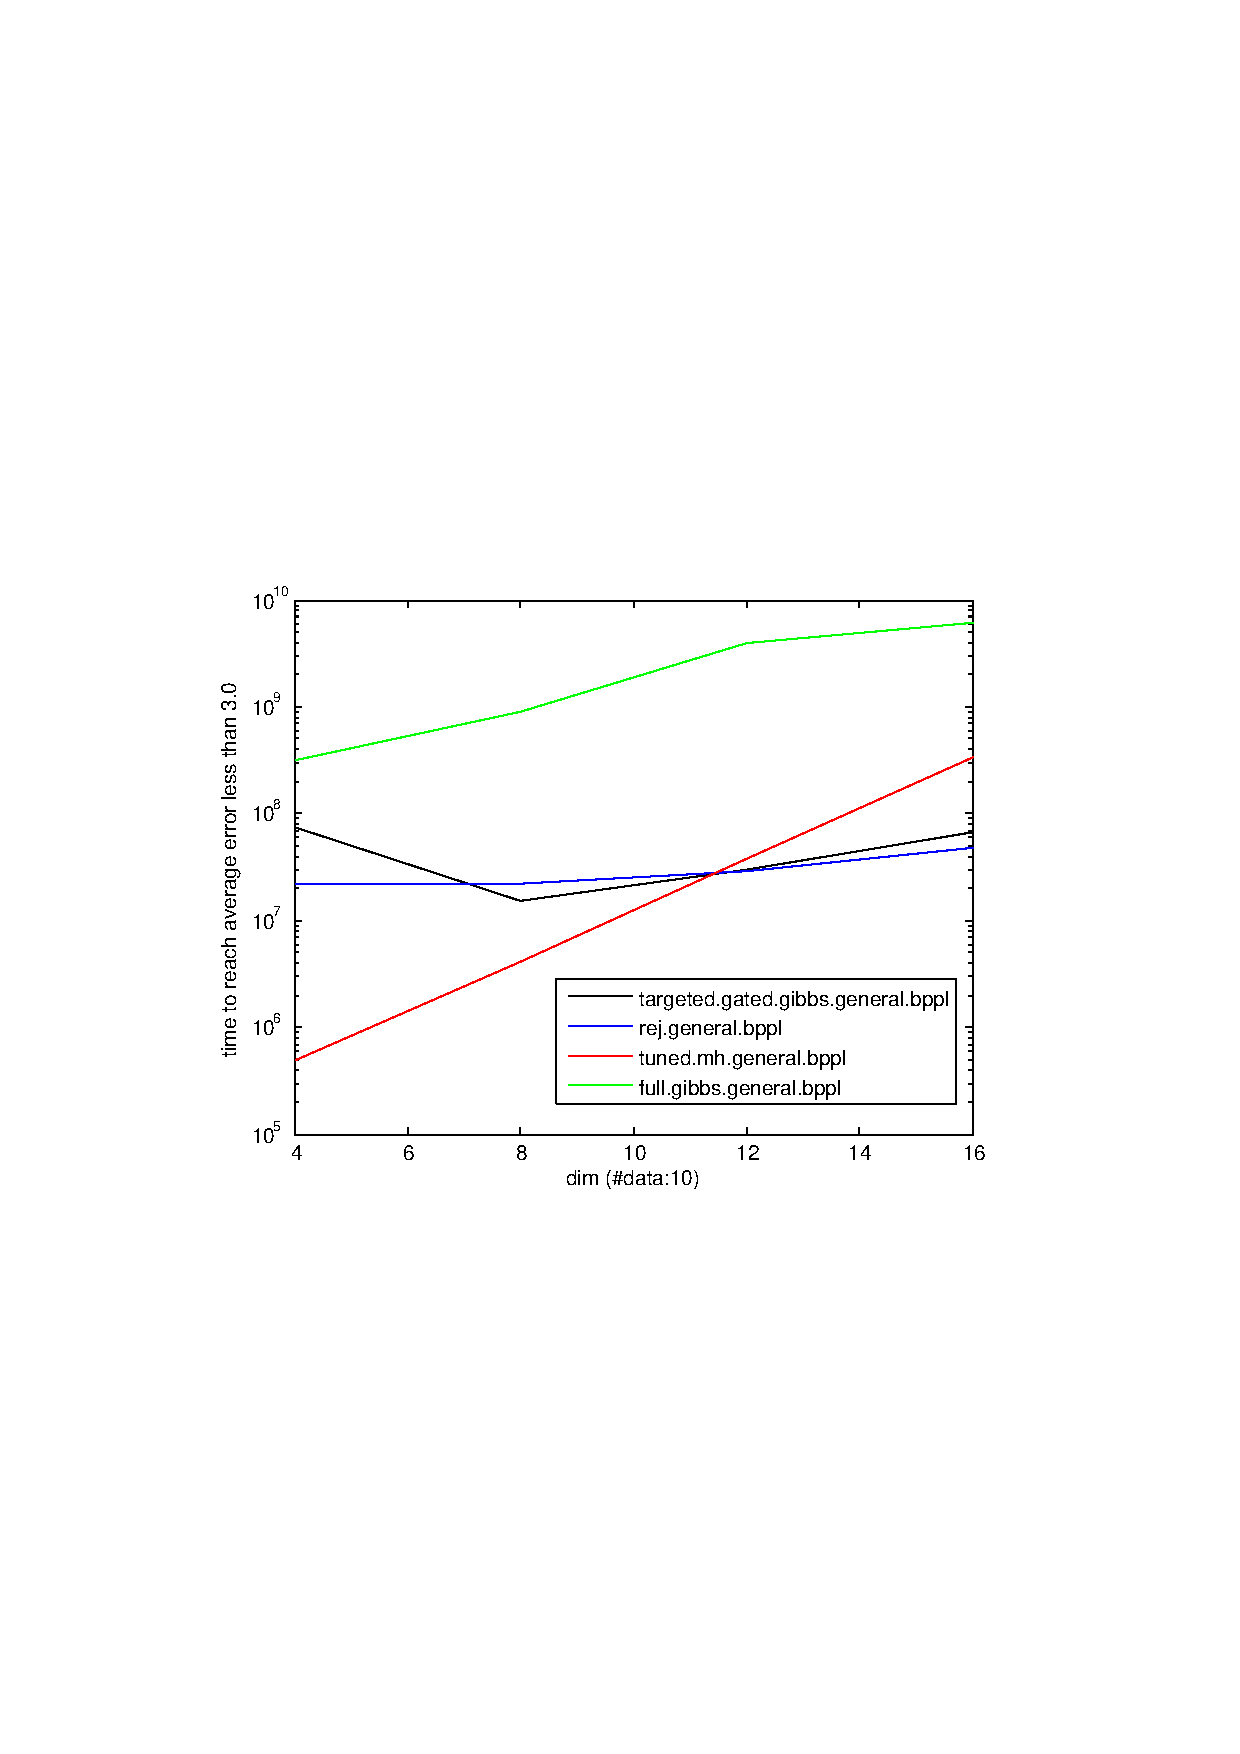
\includegraphics[width=1.2\textwidth]{pic1/dimAnalysisData10.pdf}
%\vspace{-6mm}
\caption{...}
\label{fig:pref}
%\caption{\footnotesize .} 
%\vspace{4mm}
\end{figure}

\begin{figure}%[t!]
\centering
\includegraphics[width=1.2\textwidth]{pic1/DimAnaysisData12Itr3.pdf}
%\vspace{-6mm}
\caption{itr 3; 1min; 2min...\\Seems to good to be real!}
\label{fig:pref}
%\caption{\footnotesize .} 
%\vspace{4mm}
\end{figure}


\begin{figure}%[t!]
\centering
\includegraphics[width=1.2\textwidth]{pic1/DataAnalysisDim10ErrThr3Itr3GrndTruth1MaxWait2.pdf}
%\vspace{-6mm}
\caption{itr 3; 1min; 2min...}
\label{fig:pref}
%\caption{\footnotesize .} 
%\vspace{4mm}
\end{figure}

\begin{figure}%[t!]
\centering
\includegraphics[width=1.2\textwidth]{pic1/dataAnalysis6GTbppl.pdf}
%\vspace{-6mm}
\caption{itr 3; 1min; 2min...}
\label{fig:pref}
%\caption{\footnotesize .} 
%\vspace{4mm}
\end{figure}

\newpage
\section{MMM}
\begin{figure}%[t!]
\centering
\includegraphics[width=1.2\textwidth]{pic1/DataAnalysisMMMgtruth6Wait3Min005Thr.pdf}
%\vspace{-6mm}
\caption{itr 3; 6min; 3min...}
\label{fig:pref}
%\caption{\footnotesize .} 
%\vspace{4mm}
\end{figure}

\begin{figure}%[t!]
\centering
\includegraphics[width=1.2\textwidth]{pic1/MMMdimAnalysisData6.pdf}
%\vspace{-6mm}
\caption{itr 3; 6min; 3min...}
\label{fig:pref}
%\caption{\footnotesize .} 
%\vspace{4mm}
\end{figure}


\begin{figure}%[t!]
\centering
\includegraphics[width=1.2\textwidth]{pic1/DimAnalysisData8Itr5GT8minTest4minT01MMM.pdf}
%\vspace{-6mm}
\caption{Ground-Truth is estimated by rejection sampling for 8 mins. In each dim/data setting, each algorithm is averaged over 5 runs. If in 4 mins has not reached the error threshold 0.1 it is discarded.}
\label{fig:pref}
%\caption{\footnotesize .} 
%\vspace{4mm}
\end{figure}
\end{document}